\section{Implementation on seafloor data}

The landing algorithm is applied to a $500$\,m section of high resolution seafloor laser bathymetry data collected on the southern slopes of the Takuyo Daigo seamount between depth of 1379 and 1429\,m. The data was obtained by the AUV BOSS-A using the same mapping system described in Section ~\ref{sec:algo}. In order to perform the analysis, the data is split into twenty $25$\,m long submaps as illustrated in Fig~\ref{f:mehul24}. The northern part of the transect (submaps 1 to 9) is gently sloped with relatively flat, exposed manganese crusts. The  southern parts of the transect (submaps 10 to 20) is more steeply sloped with a higher degree of rugosity~\cite{Thornton2013l,Bodenmann2016}. The algorithm was applied to determine the most appropriate landing coordinate and heading within each submap for the vehicle parameters given in Table~\ref{t:table2}. 

	
\begin{figure}[!ht]
\centering
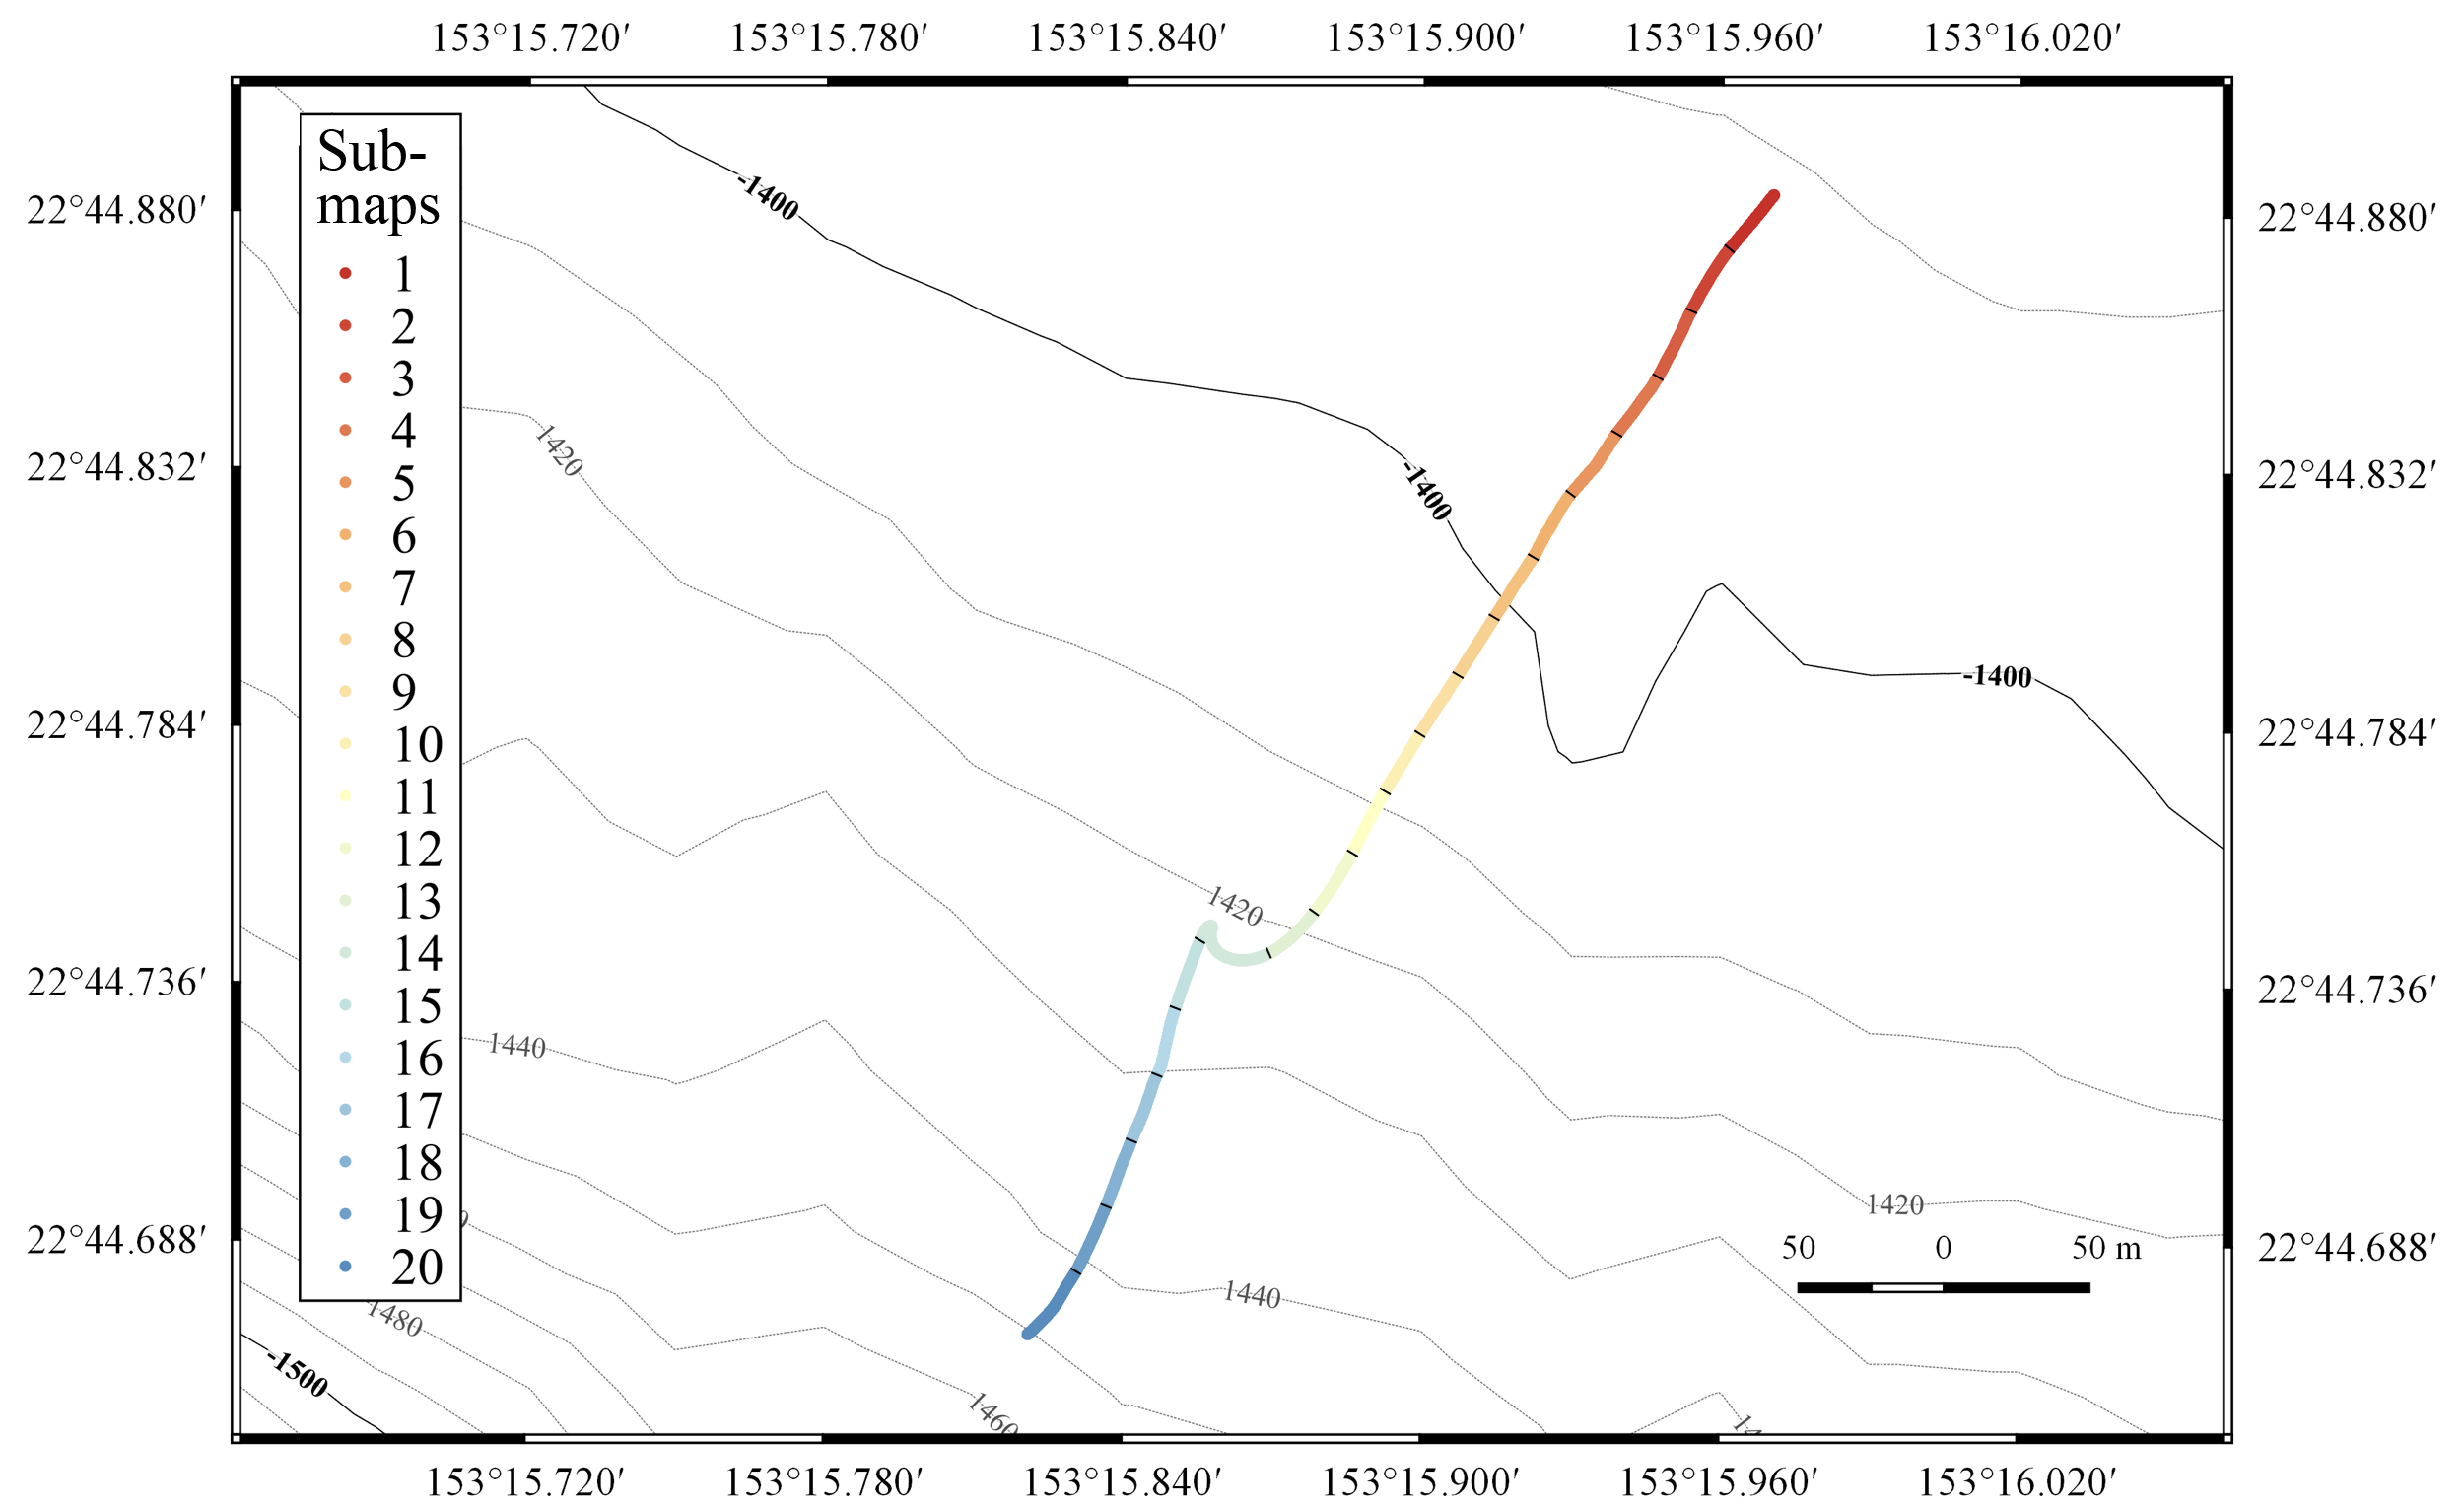
\includegraphics[width=6.5in]{./images/mehul24_BT.png}
\caption{Vehicle trajectory at Takuyo Daigo seamount where the algorithm is implemented on twenty $25$\,m long submaps}
\label{f:mehul24}
\end{figure}

\begin{figure}[!ht]
\centering
\subfloat[Properties and landing costs determined for the sites selected within each submap\label{sf:mehul25}]{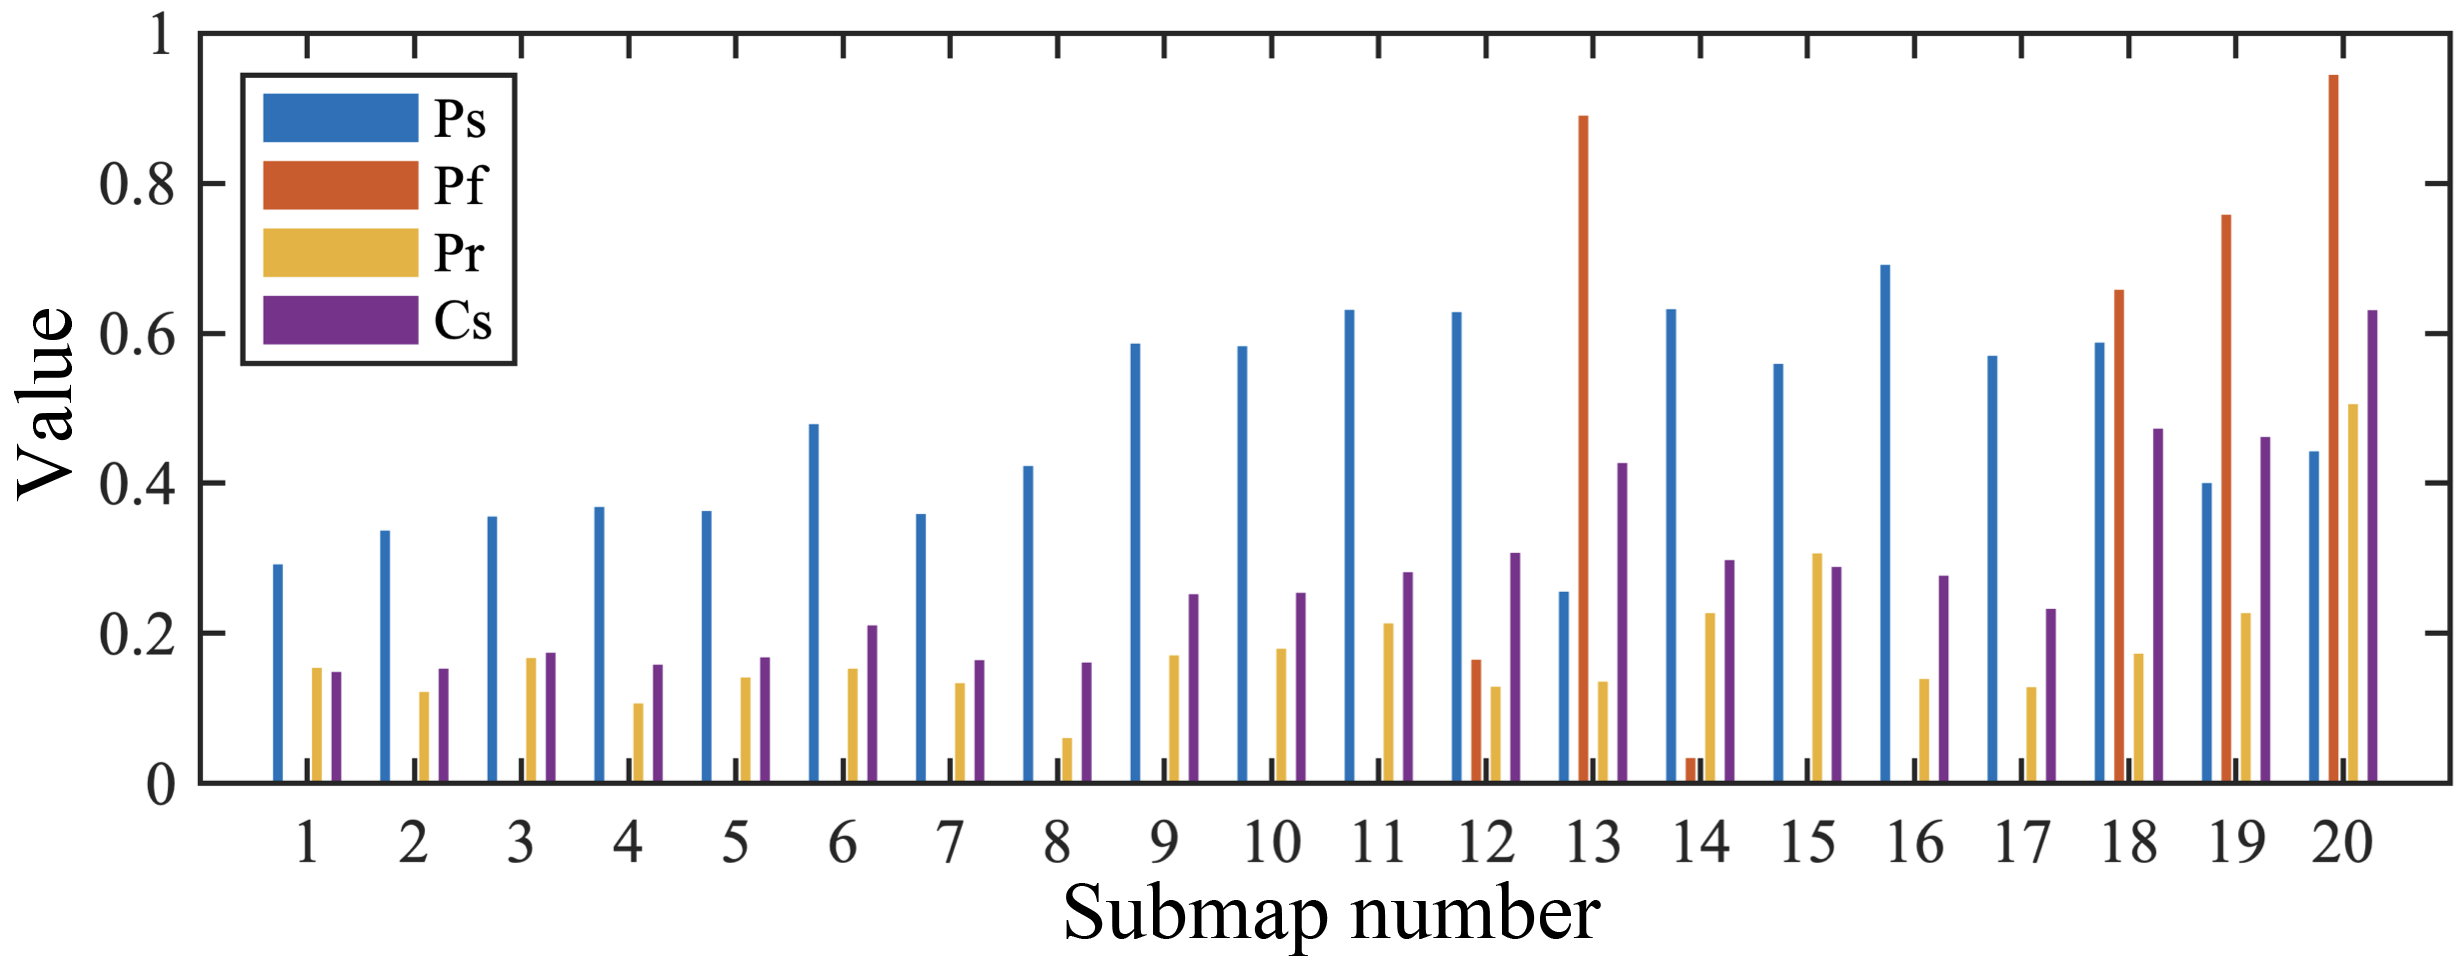
\includegraphics[width=5.5in]{./images/mehul25_BT.png}}\quad
\subfloat[Landing headings for the sites selected within each submap\label{sf:mehul26}]{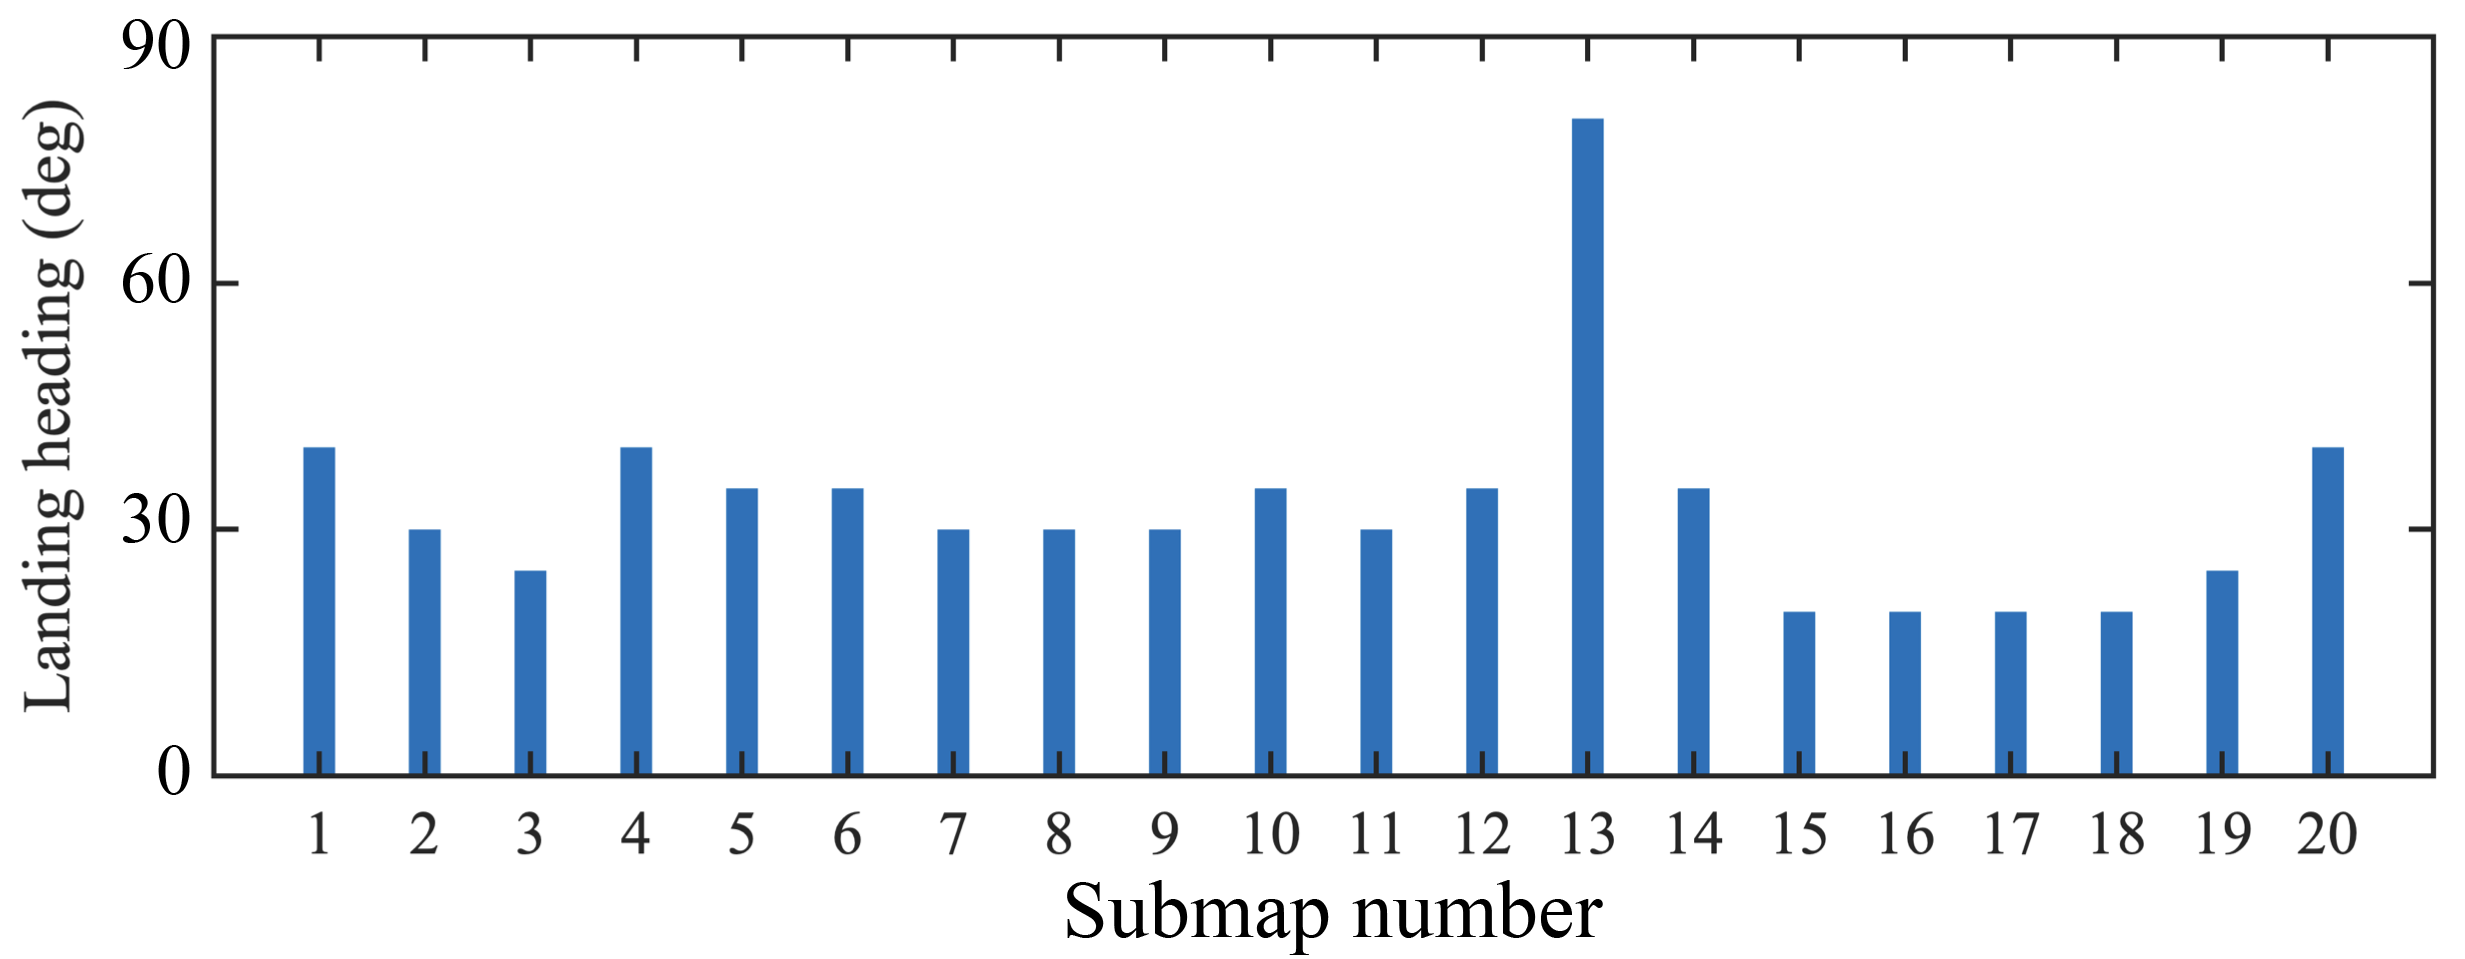
\includegraphics[width=5.5in]{./images/mehul26_BT.png}}
\caption{Characteristics of the landing sites determined by the algorithm for the submaps analysed in this work.}
\end{figure}

The algorithm selected landing sites in each submap, the properties of which can be seen in Fig~\ref{sf:mehul25}. The landing heading for each patch is close to the mapping heading due to the narrow swath of the bathymetry as shown by Fig~\ref{sf:mehul26}. This is clearly visible for the submaps shown in Fig~\ref{f:mehul27}. The sites towards the south of the transect (submaps 10 to 20) have higher landing costs than the transects towards the north of the transect (submaps 1 to 9) with larger values of Ps and Pr due to the increased steepness and rugosity. Fig~\ref{f:mehul27}a shows Submap $XX$, which has a low landing cost due to the wide swath and gently sloping smooth surface. Submap $YY$ (Fig~\ref{f:mehul27}b) shows a narrow landing area due to reduced mapping swath while turning on an smooth, gently sloping area of the seafloor. Submap $ZZ$ (Fig~\ref{f:mehul27}c) towards the lower end of the transect has a narrow landing area on an area with high rugosity and a steep slope, resulting in a high landing cost. Fig~\ref{f:mehul28} shows the locations of each landing site identified in the submaps with their Cs values.

\begin{figure}[!ht]
\centering
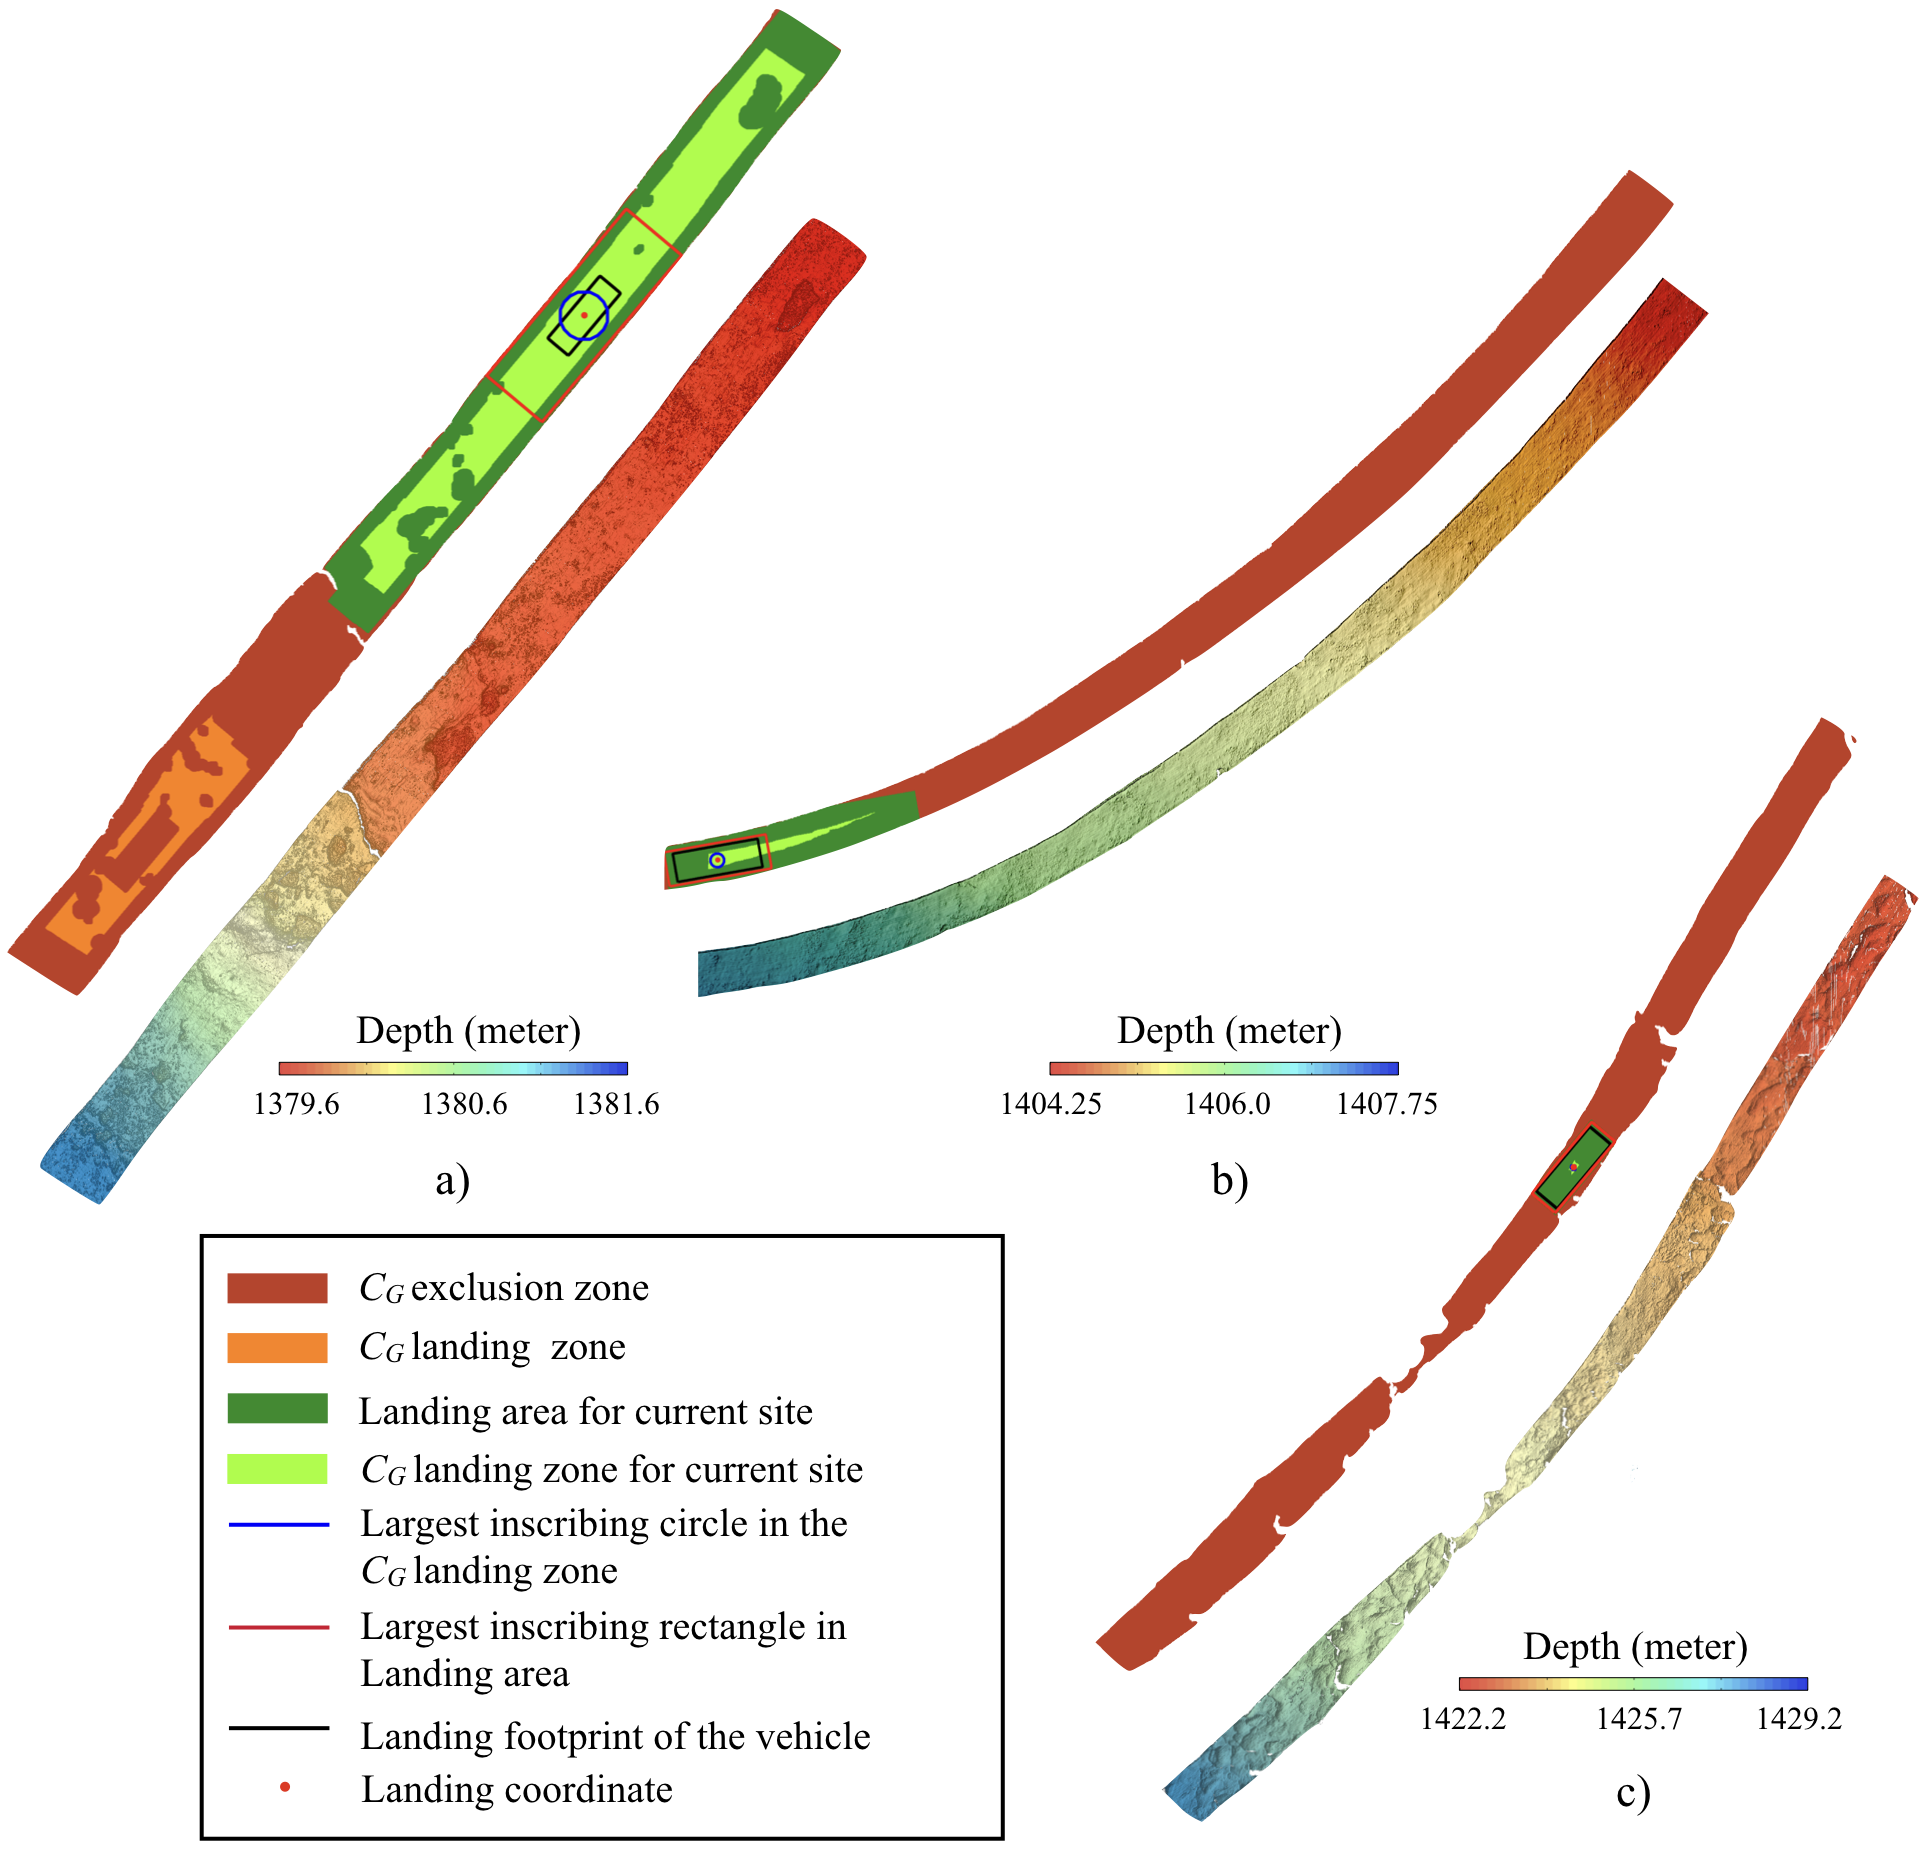
\includegraphics[width=\textwidth]{./images/mehul28.png}
\caption{Landing cost for sites identified}
\label{f:mehul27}
\end{figure}

\begin{figure}[!ht]
\centering
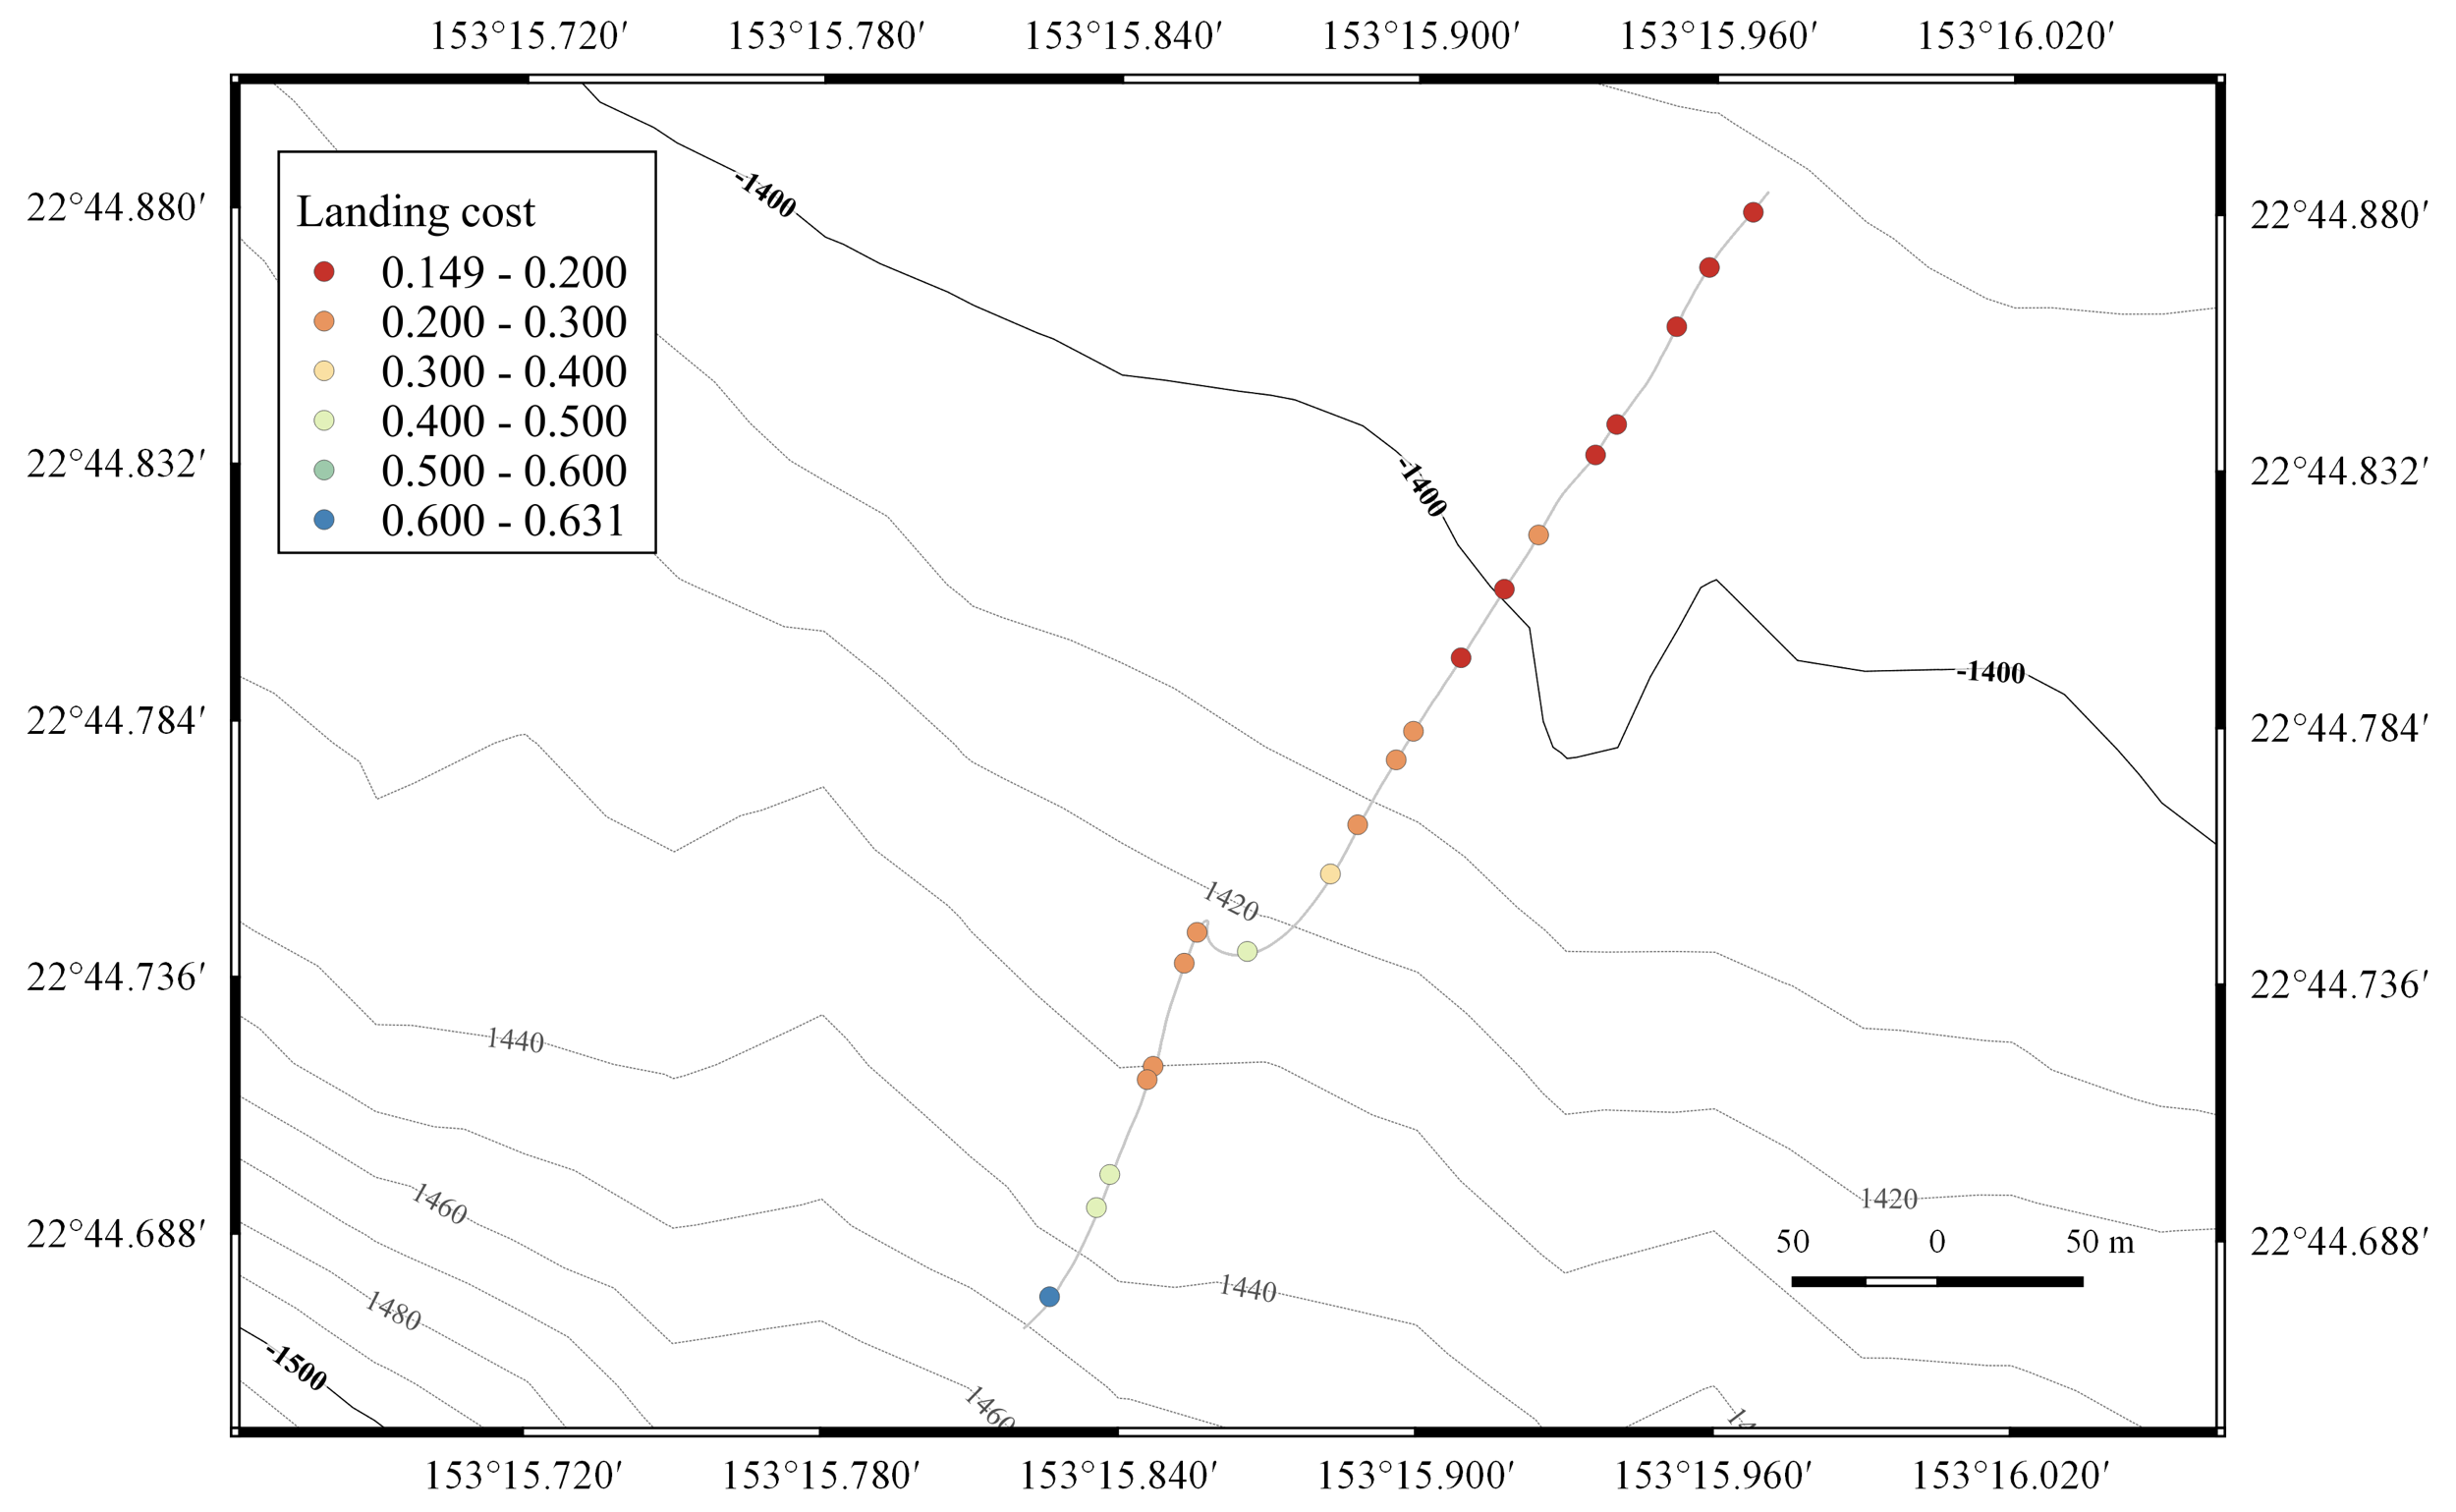
\includegraphics[width=6in]{./images/mehul27.png}
\caption{Landing cost for sites identified}
\label{f:mehul28}
\end{figure}

\begin{table}[!ht]
\centering
\caption{Results of analysis on mapped bathymetry}
\begin{tabular}{  |c c c c c|}
\hline
\textbf{Area surveyed} & \textbf{Number of sites} & \textbf{Mean landing cost} & \textbf{Landing cost range} & \textbf{Landing cost Std. Dev.}\\ \hline 
$794.4$ sq.m. & $754$ & $0.28$ & $0.15 - 0.63$ & $0.13$ \\
\hline
\end{tabular}
\label{t:table6}
\end{table}